\section{Circuit Design}

The circuit design and schematic realization of the BRD1 sub-board of the device is discussed in the following sections. This includes sections on the DDS signal generator stage, the current driver stage, the output multiplexer, as well as discussions on power supplies, digital interfacing, and clock generation.

\begin{figure}
\centering
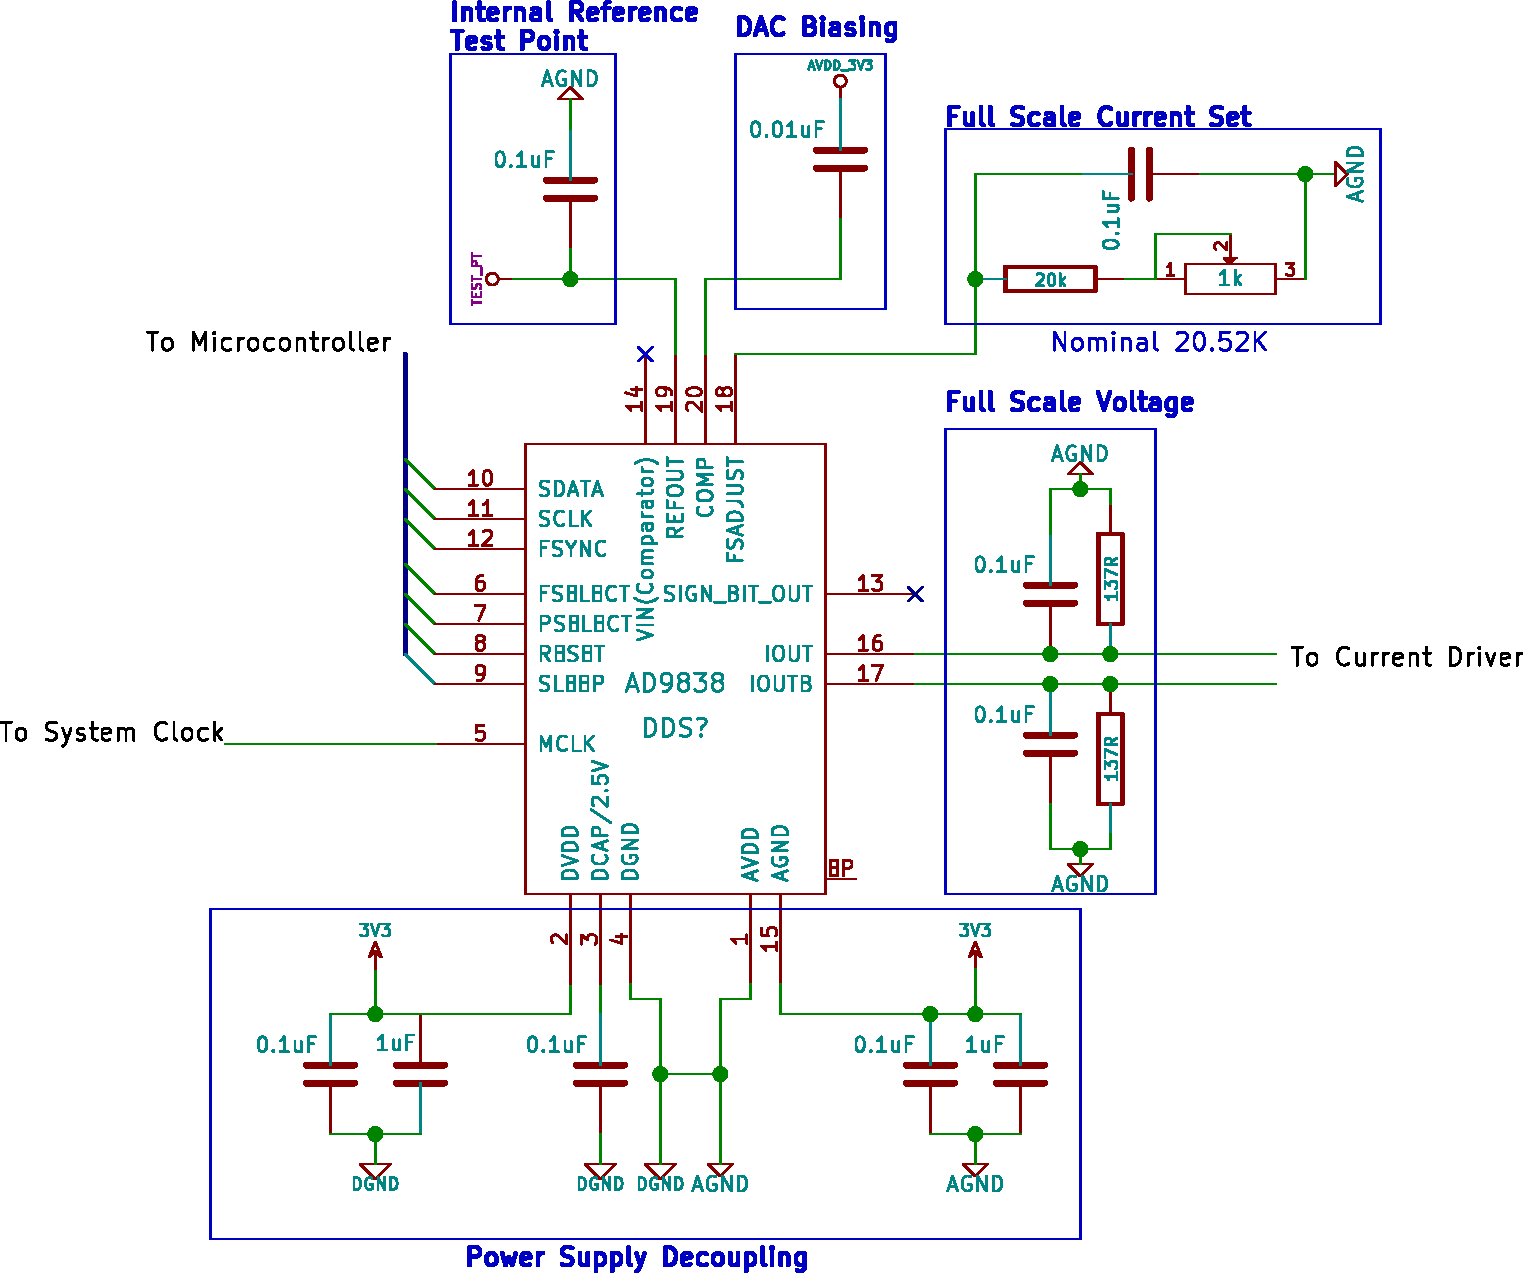
\includegraphics[width=0.9\textwidth]{../assets/images/DDS_Stage/DDS_stage_big}
\caption{Annotated schematic diagram of the DDS stage of the device. The AD9838 is the circuit element labeled DDS1. The pin names as well as pin numbers are indicated on the component.  Full Scale Current and Full Scale Voltage are used to set the input signal into the current driver stage, the functionality is discussed in Section \ref{sec:circuit_subs:dds_stage}. Power Supply decoupling is required for all power supply pins in order to minimize spurious pcb and power supply noise from bleeding into the signal, decoupling best practices are discussed in Section \ref{sec:pcb_subs:decoupling}. The internal reference pin outputs the an internal voltage referense used by the DDS, used in this design as a test point. }
\label{fig:dds_stage_main_fig}
\end{figure}


\subsection{DDS Stage}
\label{sec:circuit_subs:dds_stage}


\newthought{The first component in the TDCS driver signal chain} is the {\bf D}irect {\bf D}igital {\bf S}ynthesis ({\bf DDS}) device. The DDS replaces a microcontroller and a {\bf D}igital-{\bf A}nalog Convert ({\bf DAC}) to produce sinusoidal and triangular voltage signals in a single device.  The DDS device is designed by the manufacturer to produce a fixed signal at a digitally selectable frequency, this limits possible output options, but the integrated design limits noise, power, and reduces component count vs a discrete system. A DDS works by increasing the number stored in a memory register (phase accumulator) with every clock cycle, the number stored in the register is used to lookup a code stored in a static "lookup table" that corresponds to the output code for the integrated DAC. By choosing the size of the numerical jump that the phase accumulator undergoes every clock cycle, you can adjust the frequency through a digital "control word" 

\begin{marginfigure}[-5\baselineskip]
\framebox{\begin{minipage}[h]{1\columnwidth}
\end{minipage}}
\caption{Simplified diagram of a DDS. The control word selects the frequency of the output signal, a larger control word means a larger advancement in the phase accumulator with every clock cycle, and it takes fewer clock cycles to run through the values stored in the lookup table. A larger control word translates to a larger frequency with the relation $f = \frac{M\cdot f_c}{2^n},$ where $f_c$ is the system clock frequency and $n$ is the bit depth of the accumulator (see sidenote \ref{sidenote:bit_depth})}

\end{marginfigure}



There are a variety of DDS components on the market, they are differentiated by primarily by type and number of outputs, its noise profile, the frequency limits, power consumption, and bit depth \sidenote[][]{\label{sidenote:bit_depth} There are two bit depths that are important from a design perspective. The phase accumulator bit depth (the number of discrete steps to complete one cycle) determines the frequency resolution of the DDS. The DAC output bit depth determines the number of discrete "output modes" that the DDS can utilize to produce a signal. Typically the DAC bit depth is smaller than the phase accumulator, this means that the DDS may output the same voltage for several sequential phase steps which creates phase noise} There are also a number of other features that could be useful in certain applications, but were not considered for this implementation. For further discussion of DDS component selection refer to Section \ref{sec:components_subs:AD9838} 

Providing an output current that can both be negative or positive relative to local ground can be accomplished in several different ways. DDS outputs can either be bipolar, complimentary, or single ended, each requiring a different type of output coupling to achieve true bipolar output (see Section\ref{sec:components_subs:AD9838} for more information). The AD9838 provides complimentary current outputs, which allows for higher speeds than a voltage-output dds, and conveniently couples to the current driver stage (see Section \ref{sec:circuit_subs:vtoi}) to provide a symmetrical output signal. Complimentary current DDS devices supply the output waveform on two seperate pins (OUTA and OUTB), as the phase accumulator progresses through the steps, the output on OUTA increases from I$=0$ to $\text{I} = \text{I}_\text{Full Scale}$ while the output on OUTB decreases from $\text{I} = \text{I}_\text{Full Scale}$ to $\text{I} = 0$ over the same interval\sidenote[][]{The full scale current of the AD9838 is set with an external resistor, following the equation $\text{I}_\text{Full Scale} = 18 \times \frac{1.14\text{V}}{\text{R}_\text{ set}(\text{k}\Omega)}.$ With $\text{R}_\text{ set} = 20.52 \text{k}\Omega$, $\text{I}_\text{Full Scale} = 1\text{mA}$}. By taking the difference between these two outputs, a full bipolar output can be reconstructed from a single-ended (only positive voltages) complimentary DDS. A partial schematic of the AD9838 and supporting components is shown in Fig \ref{fig:dds_stage_main_fig}

This complimentary current output must be voltage coupled in order to work with the high input-impedance driver stage. This is accomplished by placing a resistor from the current output to ground, using Ohm's law and the given full-scale current, the full-scale voltage can be easily calculated for a given shunt resistor (In this design, $1\text{mA}$ across $137\Omega$ gives $.137\text{V}$ Peak). The AD9838 can operate within specification (output compliance) at output levels of up to $0.8\text{V}$ Peak.

Digital Control lines are used to interface with the device. The AD9838 has 3 lines dedicated to serial communication (Indicated in Fig. \ref{fig:dds_stage_main_fig} as {\bf~SDATA}, {\bf~SCLK}, and {\bf~FSYNC}) which are used for loading frequency control words and otherwise setting the operating parameters of the device. The {\bf~FSELECT} and {\bf~PSELECT} pins allow for rapid switching between stored frequencies and phase offsets (this functionality can be achieved through the serial data lines but at a much lower switching rate). {\bf~SLEEP} and {\bf~RESET} control the power state of the device. {\bf~MCLK} is the digital sampling clock input for the AD9838 (clock source is discussed in Section \ref{sec:circuit_subs:clock} )

All integrated circuits used are required to be decoupled from the power supply through the use of decoupling capacitors (capacitors placed between the power supply pin and ground) that filter high frequency noise and other unwanted spurious noise that can leak through the power supply. Power Supply decoupling is discussed in Section \ref{sec:pcb_subs:decoupling}



\begin{figure}[h]
\centering
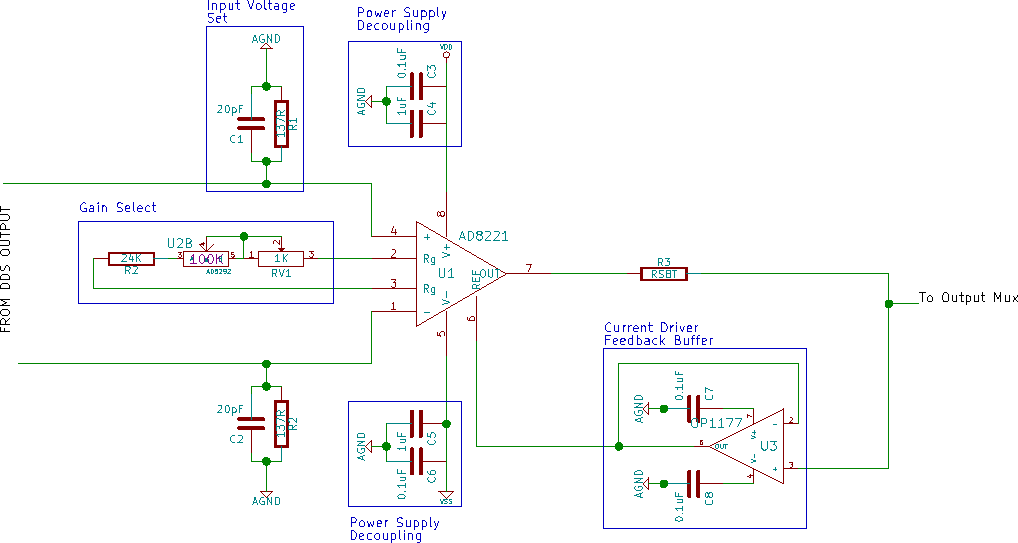
\includegraphics[width=0.9\textwidth]{../assets/images/Current_Stage/currentstage}
\caption{This section of the schematic shows the current driver stage of the device. Resistors R$1$ and R$2$ set the input voltage level to $.137$V from a $1$mA input current while C$1$ and C$2$ are noise filtering capacitors (described in Section \ref{sec:circuit_subs:dds_stage}). U$1$ is the AD8221 instrumentation amplifier, used to source the current for the rest of the device. C$3$-C$8$ are power supply decoupling capacitors described in Section \ref{sec:pcb_subs:decoupling}. U$2$B (the digital side of the component, U$2$A is not shown here) is the digital potentiometer that controls the gain of U$1$, R$2$ sets the gain ceiling and RV$1$ is a trimming potentiometer used to correct for resistor errors in R$2$, and U$2$B. $U3$ is an operational amplifier that acts as a feedback buffer. $R3$ sets current for TDCS measurements, it is replaced with a digital switch and multiple resistor values in order to have a larger range of selectable currents (Shown in Fig. \ref{fig:range_sel} )}
\label{fig:vtoi_circuit}
\end{figure}




\subsection{Current Driver Stage}
 \label{sec:circuit_subs:vtoi}
 
 
 
\newthought{At the heart of the TDCS current driver is the AD8221 Instrumentation Amplifier}. An instrumentation amplifier is a type of differential amplifier (the output is the difference between the two inputs) with a number of additional benefits, it has an extremely high input impedance, high common-mode rejection, and minimal dc offset (see section XXXX for information on these parameters). Fig \ref{fig:vtoi_circuit} is a diagram of this part of the device. Ignoring the gain of the amplifier for now, the output of the AD9838 is the difference between the two input signals that are driven by the DDS, as the DDS sends complimentary currents (as one increases the other decreases), this difference reproduces a true bipolar output signal. A reference resistor (later expanded to a switch and bank of resistors for range selection), sets the current that will flow to the rest of device and ultimately to the subject. The reference resistor alone does not make a stable current source, as the impedance of the rest of the system will decrease the voltage drop across the reference resistor and change the current. However, by adding a feedback loop using the reference pin of the AD8221, the output of the amplifier is shifted up in order to compensate for the impedance in the rest of the system. Because the feedback loop will track the output very quickly (An operational amplifier is used to buffer the feedback signal), the current source will provide a stable current that only depends on the reference resistor and not the impedance in the rest of the system. The output voltage of the AD8221 will subsequently increase in order to compensate for the feedback voltage, $\text{V}_\text{out} = \text{V}_\text{R} + \text{V}_\text{bias}$. $V_\text{R}$ is forced to be $\text{Gain}\times(\text{V}_\text{IN1} - \text{V}_\text{IN2})$. The amplifier can keep producing the voltage necessary to source the desired current until it is close to the supply voltage ($\pm12$V). This limitation determines the maximum output current achievable for a given probe impedance.

The current is set by the reference resistor, but can also be affected by the gain of the amplifier. At $\text{G} = 1$ the difference between the output and the reference pin voltage is forced to be the difference between the two input signals, this voltage sets the current ($\text{I}_\text{out} = \text{V}_r/\text{R}_\text{ref}$), if $\text{V}_r$ is increased by increasing the gain, the current will increase proportionally. The gain on the AD8221 is set via a single external resistor ($R_g$), and is given by 
\begin{equation}
G = 1 + \frac{49.4\text{k}\Ohm}{\text{R}_g}.
\end{equation}
. In order to make the gain externally controllable, we use an AD$5292$ digital potentiometer instead a constant resistor. Digital potentiometers have a constant linear step in their resistance, the AD5292 has 1024 steps, and the worst case error for each step is $\pm1$ step. Because  at larger gain values, the difference between 2 sequential resistor value can increase the gain significantly. In order to avoid issues from digital potentiometer error, we limit the gain of the system by using a set resistor in addition to the digital potentiometer. By using a $24.7\text{K}\Ohm$ resistor, the gain is hardware limited to 3x, a $100\text{K}\Ohm$ digital potentiometer is used to select an operating gain between $1.4$x and $2.8$x. This design allows the use of the entire digital potentiometer range, with $G=1.4$ at $R_\text{DPOT} = 98.8\text{K}\Ohm$ and $G=2.8$ at $R_\text{DPOT} = 2.74\text{K}\Ohm$


\begin{figure}[h]
\centering
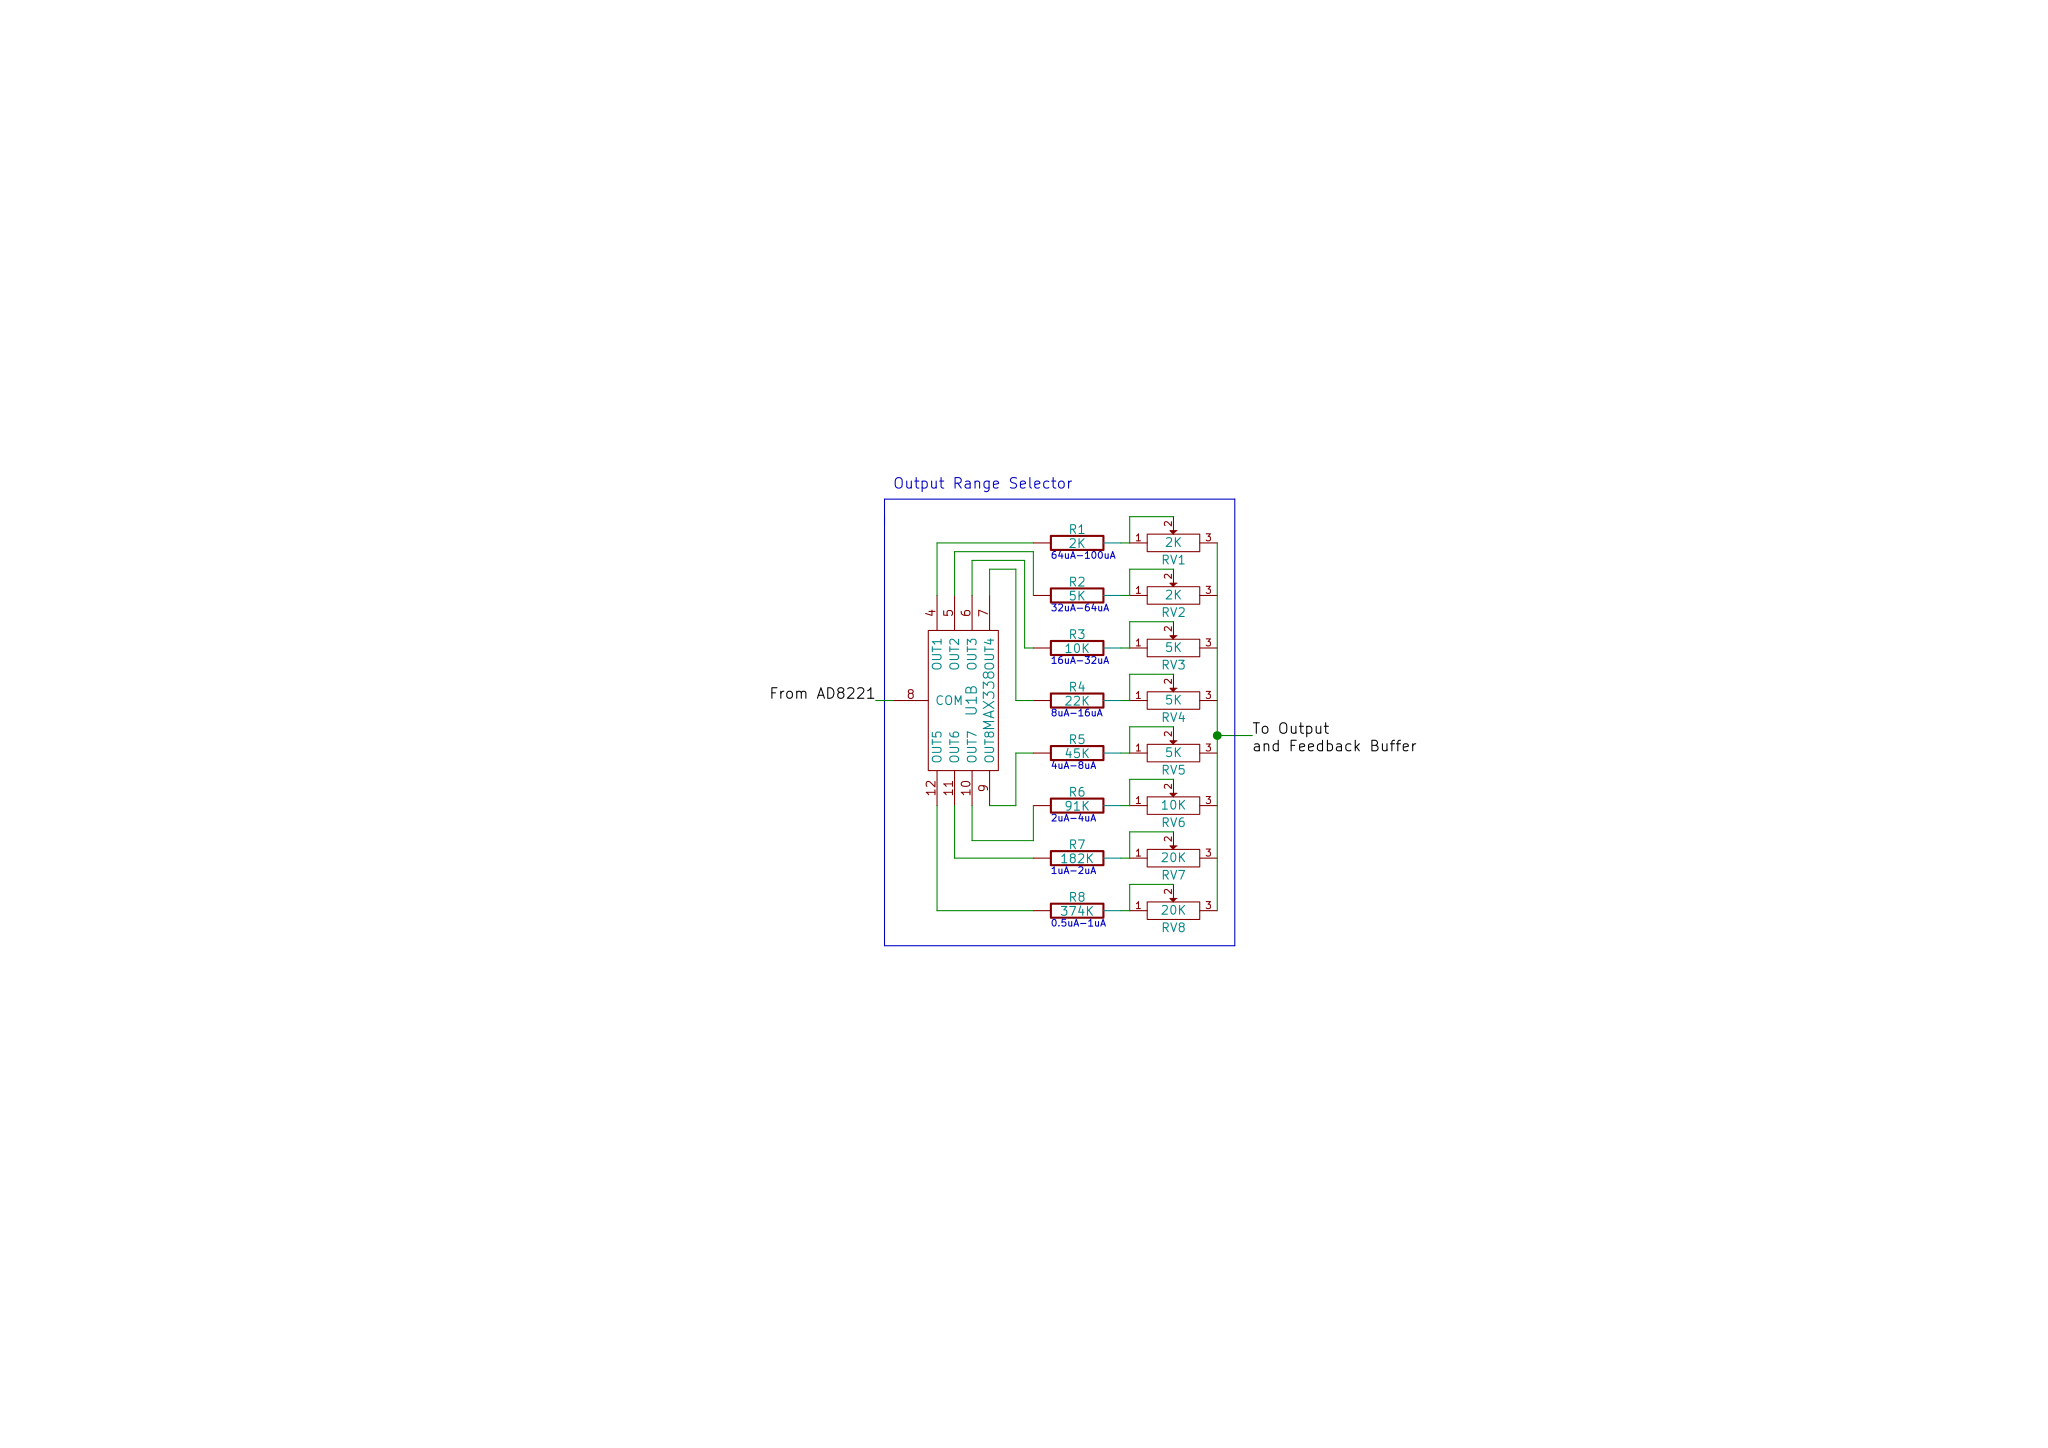
\includegraphics[width=0.9\textwidth]{../assets/images/Range_Select/range_select}
\caption{Diagram of the output range selector. R1-R8 are the range resistors and RV1-RV8 are trimmer potentiometers. U1B (The Digital control side of the same component - U1A is not shown on this diagram) is the MAX338 8:1 multiplexer. }
\label{fig:range_select}
\end{figure}

\subsection{Range Selection}

In order to still have a wide output range with the design limited gain of the AD8221, we use a 8-way analog multiplexer in order to select between one of eight different current set resistors. With 8 different selectable ranges and a maximum 2x increase in gain, we can achieve a range of $0.5\mu\text{A}$ to $100\mu\text{A}$ guaranteed for probe impedances of up to $200\text{K}\Ohm$. In order to compensate for resistor tolerances and spurious resistance in the multiplexer (Up to $400\Ohm$ worst case), trim potentiometers are used to fine tune the current output for each range setting. With the values specified in previous sections, the input signal to the AD8221 is $.137$V, with a gain of $1.4-2.8$x, this translates to $.2$V to $.4V$ to use for current generation,

\begin{table}
\begin{tabular}{c | c c |c| c}
\multicolumn{1}{p{1.75cm}}{\centering Nominal Resistance \\ (K$\Ohm$)} &
\multicolumn{1}{p{1.75cm}}{\centering Min Current \\ ($\mu$A)} & 
\multicolumn{1}{p{1.75cm}}{\centering Max Current \\ ($\mu$A)} &
\multicolumn{1}{p{1.75cm}}{\centering Set Resistance \\ (K$\Ohm$) } &
\multicolumn{1}{p{1.75cm}}{\centering Trim Pot Resistance \\ (K$\Ohm$) } \\
\hline
384 & 0.5 & 1 & 374 & 20 \\
192 & 1 & 2 & 182 & 20 \\
96 & 2 & 4 & 91 & 10 \\
48 & 4 & 8 & 45 & 5 \\
24 & 8 & 16 & 22 & 5 \\
12 & 16 & 32 & 10 & 5 \\
6 & 32 & 64 & 5 & 2 \\
3 & 64 & 100 & 2 & 2 \\
\end{tabular}
\caption {Nominal resistance for a given current range, as well as the selected static resistance and trim pot values}
\end{table}

The multiplexer used is a MAX338 8-way multiplexer. 


\subsection{Output Interfacing}

The TDCS driver is designed to operate with up to 256 probes using stackable daughter-boards, the limitation of available multiplexers means that several are needed in order to get 256 switching options. The TDCS main-board starts the process with two 8-way multiplexers (one each for current output and current return), the daughter-boards consist of two pairs of 32 output multiplexers (each pair consists of symmetrical of input/output multiplexers) with each daughter-board accommodating a bank of 64 output probes. 

The main-board interfaces with the daughterboards in two ways. The output signals are routed to 8 two-pin Molex Connectors, each one carrying an output/return pair. Digital signals to control the daughterboards are passed through logic translators (the unique 32 output multiplexers on the daughter-boards require a lower logic voltage level than the rest of the system) on  the main-board and are connected to three sets of stackable pin headers that pass these signals along to the stacked daughter-boards. 


\begin{figure}[h]
\centering
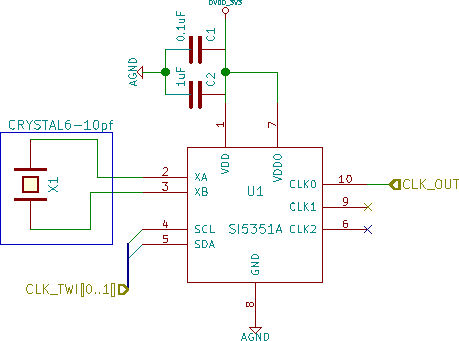
\includegraphics[width=0.9\textwidth]{../assets/images/Clock/clocksch}
\caption{Diagram of the clock generator, C1 and C2 are decoupling capacitors. X1 is a crystal oscillator. }
\label{fig:system_clock}
\end{figure}

\subsection{System Clock}

The system clock is provided by a Silicon Instruments SI5351A clock generator. This is a versatile device that only requires an external crystal oscillator to generate a clock signal. Since there is only one clocked component in the TDCS device, there is no clock routing/synchronization worries that need to be taken into account. However, to account for future developments the SI5351A has a number of different frequency generating options as well as 3 independent clock outputs. 



\subsection{Power Supply}




